% Evangelos 2009/12/19

\subsection{\label{s:mfReqb} A slice for \cLe}

As became clear in \refsect{sec:mf}, the use of a coordinate \slice\ \refeq{eq:CLEsliceSO2}
allowed explicit determination of the moving frame map \refeq{eq:CLEmf} and straightforward
determination of invariant variables \refeq{eq:invLaser}.
On the other hand \slice\ \refeq{eq:CLEsliceSO2} is defined to be orthogonal
to the group tangent of \SOn{2} restricted in the $x$-irreducible subspace of \SOn{2}
and this introduces singularities in the transformations \refeq{eq:invLaser}.
Here we will remove this restriction to a coordinate \slice\ and therefore to
an irreducible subspace and construct a moving frame by defining the slice to be orthogonal
to the group orbit at a given point in space $\slicep$. The price to pay is that it
won't be convenient to explicitly write out the transformations to invariant variables
as we did in \refsect{sec:mf}; we will instead implement the moving frame map numerically,
mapping computed trajectories to the \slice.
This is by no means a drawback. Even though the computation of invariants with the
{\mframes} is efficient, it is still computationally
prohibitive for very high dimensional flows. For, one has
to compute the invariants with computer algebra, a proccess
that works\rf{SiminosThesis} for moderate system dimension of the order of $100$,
as required for instance in truncations of \KSe\ studied in \refref{SCD07},
but does not scale well for problems with truncations of order $10,000$ as
a fully resolved $3$-D fluid simulation would easily require\rf{GibsonPhD}.
We will demonstrate in the example of \cLe\
how one can use the geometric interpretation of the {\mframes}
to simply and effectively, perform continuous symmetry
reduction in high-dimensional flows.


Specifically, we define a slice by \refeq{PCsectQ}
In our \cLe\ example we will choose a point on \reqv\ group orbit,
$\slicep  = \ssp_{\REQB{1}}$.
Each group intersects the section exactly twice,  with the
two solutions separated by $\pi$. We select the one \ESedit{
that is at the smallest Euclidean distance from $\slicep$.}
\ES{replaced: with a
smaller clockwise rotation angle into the \slice.} \ES{dropped
as I am not sure it is correct for multiparameter groups. Even
for \cLe\ it seems to imply that the slice exists on the $z$-axis,
which I think is not true: The
invariant subspaces are always within the \slice, as $\Lg_a
 \ssp =0$ for $\ssp$ in an invariant subspace.
}
Projection of \cLe\ dynamics to the slice defined in this way are
shown in \reffig{fig:CLEmfReqb1}. We see that the problems of
\reffig{fig:CLEmf} are not present in \reffig{fig:CLEmfReqb1}, since
the slice now is not defined only where the group action is not free,
that is in the set of points that are fixed by the group action. This
is the $z$-axis and as we have remarked it cannot be reached by generic
trajectories. We have to caution the reader that this is a fortuitous
event. For more general group representations symmetry reduction through
the use of a slice will be at best local as we intend to discuss
elsewhere\rf{SCD09b}. Nevertheless, using local slices defined by \refeq{PCsectQ}
to tesselate the \reducedsp\ is an optimal choice in the sense that any
failure will occur in \fixedsp\ $\Fix{\LieElrep_a}$ of some subgroup
$\LieElrep_a$.


%%%%%%%%%%%%%%%%%%%%%%%%%%%%%%%%%%%%%%%%%%%%%%%%%%%%%%%%%%%%%%%%
%computed with vaggelis/testing/flows/CLEfinalTmp.nb
\begin{figure}[ht]
\begin{center}
  (\textit{a})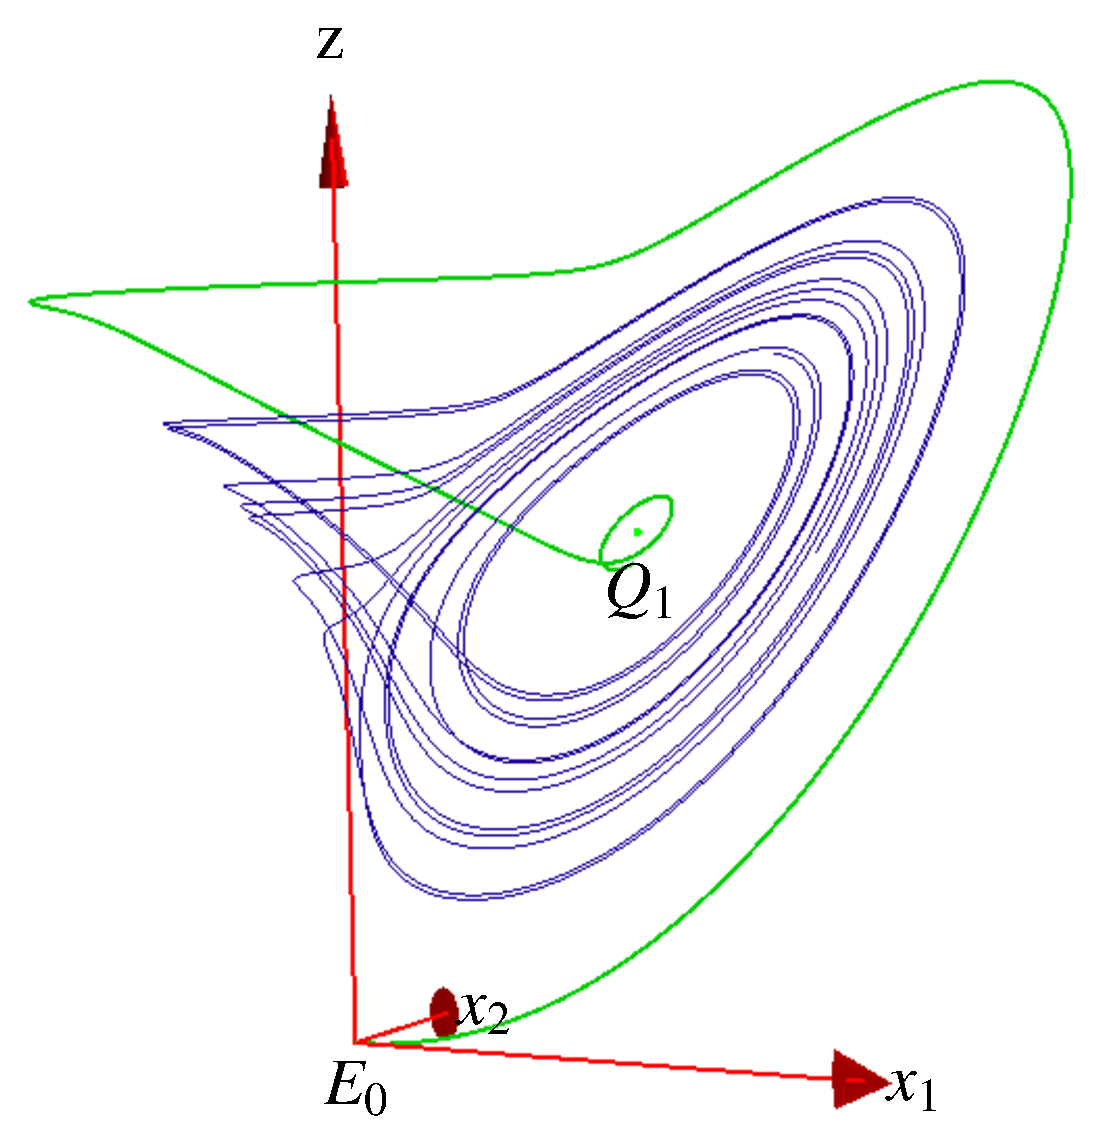
\includegraphics[width=0.35\textwidth,clip=true]{../figs/CLEmfReqb1}
~~~~(\textit{b})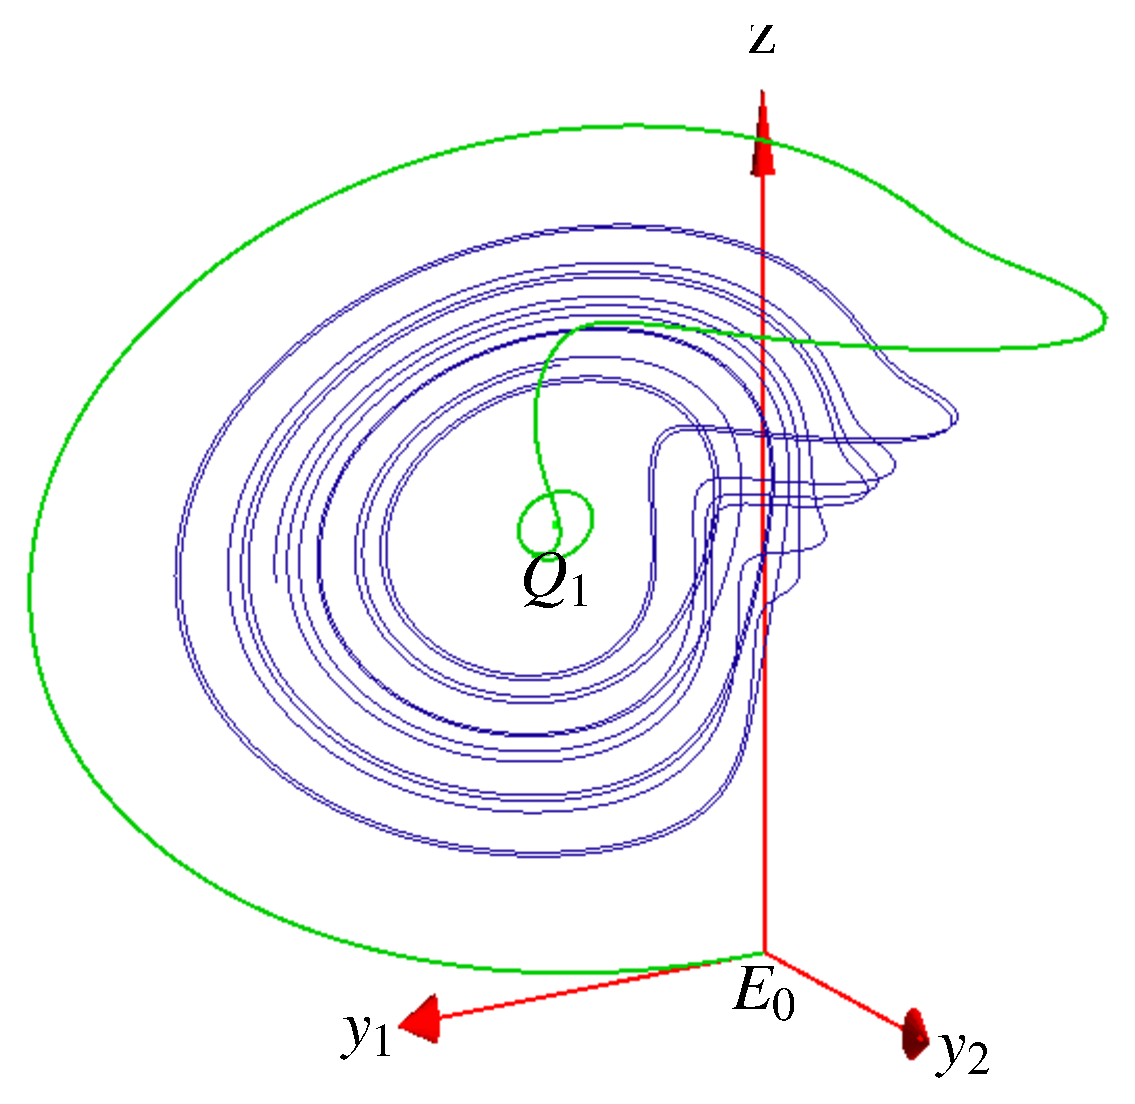
\includegraphics[width=0.35\textwidth,clip=true]{../figs/CLEmfReqb}
\end{center}
\caption{ \Statesp\
portraits of \cLe\ dynamics for $e=1/10$, $\ImrCLor=0$
in \reducedsp. We use a moving frame map to a slice orthogonal
to the group tangent at  $\slicep  = \ssp_{\REQB{1}}$. We have rescaled $x_2$ and $y_2$
for clarity.
    }
\label{fig:CLEmfReqb1}
\end{figure}
%%%%%%%%%%%%%%%%%%%%%%%%%%%%%%%%%%%%%%%%%%%%%%%%%%%%%%%%%%%%%%%%

Moreover, rotation of $\ssp$ by angle $\theta$
to the slice defined by \refeq{PCsectQ1} is a linear operation
for any given point and can be applied efficiently
even in a high dimensional space. This is especially true
for truncations of PDEs, when typically the rotation group
representation is a direct sum of irreducible
representations and one is not force to store large matrices.
Of course, the transformation is still non-linear
through the dependence on the angle and equivalent to the
explicit transformations \refeq{eq:invLaser}.


Since rotations commute with time integration, one can take a different approach:
starting with a point on the slice integrate for small but finite time and then map the
corresponding orbit segment to the section and repeat the procedure. In this setting it
is easier to distinguish between the two points of intersection of the slice and the group
orbit (for instance we can peek the one with a smaller clockwise rotation angle into the \slice)
but we get no further practical advantages. Nevertheless, in the limit of infinitesimal
time steps this procedure reveals the connection of \mframes\ method to
its continuous time counterpart of \refsect{sec:MovFrameODE}.
    \ES{I didn't see the need to write a subsection for this.}
